% ============================================================
\chapter{Span, Independence, Bases, and Coordinates}
\label{ch:span-bases-coordinates}
% ============================================================

\section*{Chapter Preview}
\addcontentsline{toc}{section}{Chapter Preview}

A small list of vectors can describe a large space. Span explains how. Linear
independence explains when no vector in the list is redundant. A basis is a
list that is just large enough to describe every vector uniquely, and
coordinates are the numbers in that description.

\section{Linear Combinations and Span}

\begin{definition}
  A \emph{linear combination} of vectors $v_1,\ldots,v_k$ is a vector of the
  form
  \[
    \lambda_1v_1+\cdots+\lambda_kv_k,
  \]
  where the coefficients $\lambda_i$ are scalars.
\end{definition}

\begin{definition}
  The \emph{span} of $v_1,\ldots,v_k$ is the set of all their linear
  combinations:
  \[
    \Span\{v_1,\ldots,v_k\}
    =
    \{\lambda_1v_1+\cdots+\lambda_kv_k:\lambda_i\in\F\}.
  \]
\end{definition}

\begin{figure}[h]
  \centering
  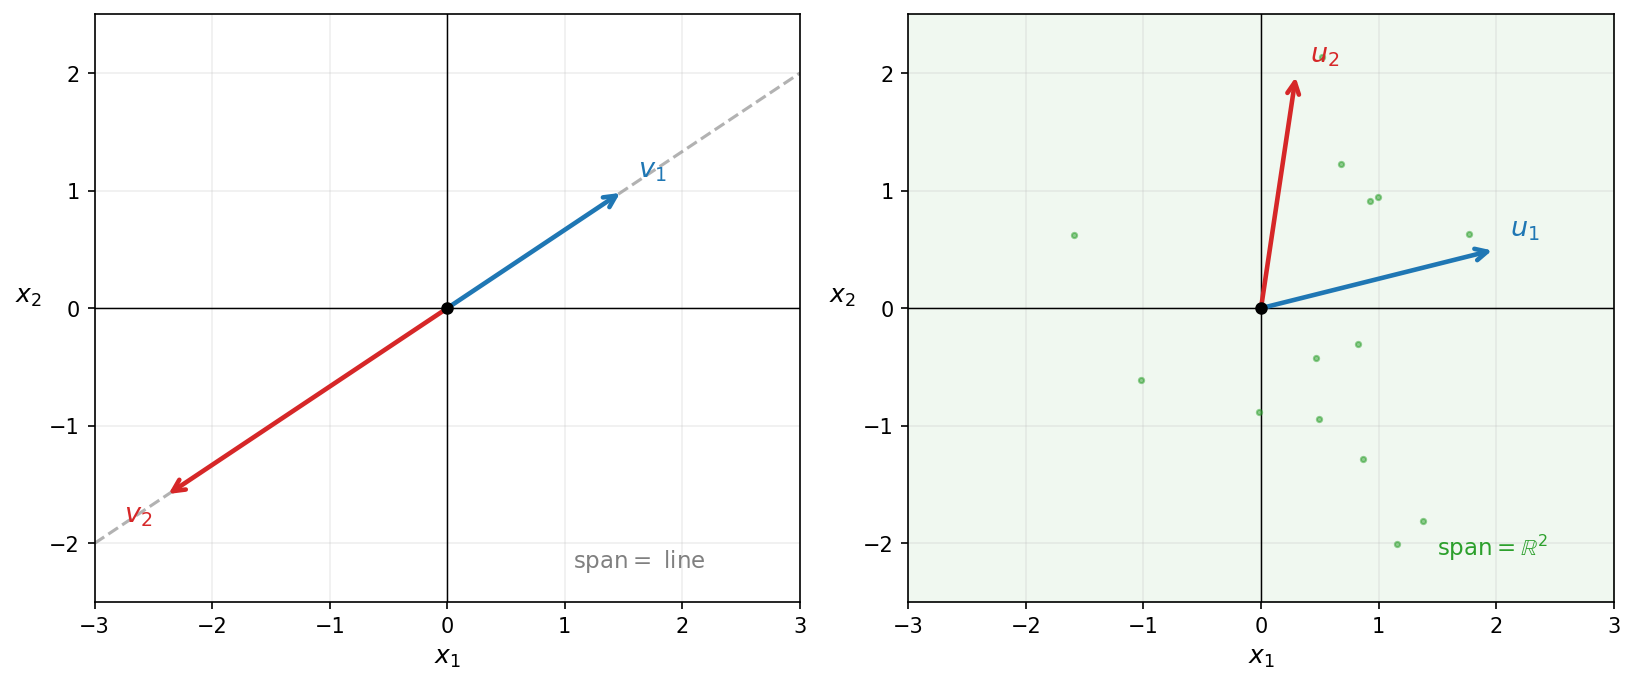
\includegraphics[width=\textwidth]{book/assets/figures/core/fig03_span.png}
  \caption{Two collinear vectors span a line. Two independent vectors in
  $\R^2$ span the whole plane.}
\end{figure}

\begin{proposition}
  $\Span\{v_1,\ldots,v_k\}$ is the smallest subspace containing
  $v_1,\ldots,v_k$.
\end{proposition}

\begin{proof}
  The span is closed under linear combinations, so it is a subspace. It
  contains each $v_i$ by taking coefficient $1$ on $v_i$ and $0$ on the
  others. Any subspace containing all the $v_i$ must contain all their linear
  combinations, so it must contain the span.
\end{proof}

\section{Linear Independence}

\begin{definition}
  A list $v_1,\ldots,v_k$ is \emph{linearly independent} if
  \[
    \lambda_1v_1+\cdots+\lambda_kv_k=0
  \]
  implies $\lambda_1=\cdots=\lambda_k=0$.
\end{definition}

If a list is not independent, then one vector is redundant: it can be written
as a linear combination of the others.

\begin{proposition}[Dependence means redundancy]
A list $v_1,\ldots,v_k$ is linearly dependent if and only if at least one
vector in the list lies in the span of the others.
\end{proposition}

\begin{proof}
If, for example, $v_j$ lies in the span of the other vectors, then
\[
  v_j=\sum_{i\ne j} c_i v_i
\]
gives the nontrivial relation $v_j-\sum_{i\ne j}c_i v_i=0$.
Conversely, suppose
\[
  c_1v_1+\cdots+c_kv_k=0
\]
with some $c_j\ne 0$. Solving for $v_j$ gives
\[
  v_j=-\sum_{i\ne j}\frac{c_i}{c_j}v_i,
\]
so $v_j$ is redundant.
\end{proof}

\section{Bases}

\begin{definition}
  A \emph{basis} of a vector space $V$ is a list of vectors that spans $V$ and
  is linearly independent.
\end{definition}

The two conditions work together. Spanning says every vector can be described.
Independence says the description is unique.

\begin{proposition}[Equivalent views of a basis]
For a finite list $b_1,\ldots,b_n$ in $V$, the following ideas are equivalent:
\begin{enumerate}
  \item the list is a spanning independent list;
  \item the list is a minimal spanning list;
  \item the list is a maximal independent list;
  \item every $v\in V$ has a unique expansion
  $v=c_1b_1+\cdots+c_nb_n$.
\end{enumerate}
\end{proposition}

This is why bases are efficient descriptions. A spanning list with redundancy
wastes coordinates; an independent list that does not span misses vectors. A
basis is exactly balanced.

\begin{theorem}[Unique coordinates]
  If $b_1,\ldots,b_n$ is a basis of $V$, then every $v\in V$ can be written in
  a unique way as
  \[
    v=c_1b_1+\cdots+c_nb_n.
  \]
\end{theorem}

\begin{proof}
  Existence comes from spanning. For uniqueness, suppose
  \[
    v=c_1b_1+\cdots+c_nb_n=d_1b_1+\cdots+d_nb_n.
  \]
  Subtracting gives
  \[
    0=(c_1-d_1)b_1+\cdots+(c_n-d_n)b_n.
  \]
  Independence forces $c_i-d_i=0$ for all $i$, so $c_i=d_i$.
\end{proof}

\section{Dimension}

\begin{definition}
  If $V$ has a basis with $n$ vectors, then $V$ is \emph{finite-dimensional}
  and $\dim V=n$.
\end{definition}

The fact that every basis of the same finite-dimensional space has the same
number of vectors is a theorem. It is what makes dimension well-defined.

\section{Python: Coordinates in a Basis}

If the basis vectors are the columns of a matrix $B$, then finding coordinates
of $v$ means solving
\[
  Bc=v.
\]

\begin{lstlisting}
import numpy as np

B = np.array([[1.0, 1.0],
              [1.0, -1.0]])
v = np.array([3.0, 1.0])

c = np.linalg.solve(B, v)
print("coordinates:", c)
print("reconstruction:", B @ c)
\end{lstlisting}

\begin{computebox}
The command \texttt{np.linalg.solve(B, v)} calls optimized numerical linear
algebra routines. Later we will learn the mathematical structure behind this
kind of computation.
\end{computebox}

\section*{Chapter Summary}
\addcontentsline{toc}{section}{Chapter Summary}

\begin{itemize}
  \item Span is the set of all linear combinations.
  \item Linear independence means no nontrivial linear combination gives zero.
  \item A basis is a spanning independent list.
  \item A basis gives unique coordinates.
  \item Dimension is the number of vectors in any basis.
\end{itemize}

\section*{Where This Appears Later}
\addcontentsline{toc}{section}{Where This Appears Later}

Coordinates and bases are the mechanism behind matrices, change of basis,
diagonalization, Fourier methods, and PCA.

\section*{Exercises}
\addcontentsline{toc}{section}{Exercises}

\subsection*{A. Theory}

\begin{exercise}
\exerciseid{3.A1}
Prove that $\R^n$ with componentwise addition and scalar multiplication is a
vector space. You may group the axioms by saying which properties follow from
the corresponding properties of real numbers.
\end{exercise}

\begin{exercise}
\exerciseid{3.A2}
Prove that the zero vector in a vector space is unique.
\end{exercise}

\begin{exercise}
\exerciseid{3.A3}
Let $A$ be an $m\times n$ matrix. Prove that
\[
  \{x\in\R^n:Ax=0\}
\]
is a subspace of $\R^n$.
\end{exercise}

\begin{exercise}
\exerciseid{3.A4}
Find the false step in this argument: ``The set
$\{(x,y):x+y=1\}$ is a subspace because the equation is linear.''
\end{exercise}

\subsection*{B. By Hand}

\begin{exercise}
\exerciseid{3.B1}
Decide whether each subset of $\R^2$ is a subspace:
\[
  \{(x,y):y=2x\},\quad
  \{(x,y):y=2x+1\},\quad
  \{(x,y):xy=0\}.
\]
Give a short reason for each answer.
\end{exercise}

\begin{exercise}
\exerciseid{3.B2}
Let
\[
  W=\{(x,y,z)\in\R^3:x-y+z=0\}.
\]
Find three nonzero vectors in $W$. Then check by hand that the sum of any two
of your vectors is still in $W$.
\end{exercise}

\begin{exercise}
\exerciseid{3.B3}
Give a vector in the set $\{(x,y,z):x+y+z=1\}$ and show directly why doubling
it leaves the set.
\end{exercise}

\subsection*{C. Python / NumPy}

\begin{exercise}
\exerciseid{3.C1}
Write a function \texttt{in\_plane(v)} that tests whether
$v_1+v_2+v_3=0$ up to tolerance. Generate random examples in the plane and
test closure under random linear combinations.
\end{exercise}

\begin{exercise}
\exerciseid{3.C2}
Write a stochastic test for the unit circle in $\R^2$. Use it to find evidence
that the unit circle is not a subspace.
\end{exercise}

\subsection*{D. Challenge}

\begin{exercise}
\exerciseid{3.D1}
Let $W_1$ and $W_2$ be subspaces of $V$. Prove that $W_1\cap W_2$ is a
subspace. Is $W_1\cup W_2$ always a subspace?
\end{exercise}

